\documentclass[captions=tableheading]{scrartcl}

\usepackage{amsmath}
\usepackage{amssymb}
\usepackage[utf8]{inputenc}
\usepackage[T1]{fontenc}
\usepackage{lmodern}
\usepackage{ngerman}
\usepackage{geometry}
\usepackage{graphicx}
\usepackage{wrapfig}
\usepackage{caption}
\usepackage{wasysym}
\usepackage[separate-uncertainty=true]{siunitx}
\usepackage{picinpar}
\usepackage{tikz}
\usepackage{float}
\usepackage{booktabs}
\usepackage{enumitem} 

\renewcommand{\figurename}{Abb.}
\usepackage[
	colorlinks=true,
	urlcolor=blue,
	linkcolor=black
]{hyperref}


%Hier Titel und so
\newcommand{\versuchnummer}{V27} 
\newcommand{\versuchname}{Der Zeeman-Effekt} 
\newcommand{\versuchdatum}{16.02.2017} 
\newcommand{\im}{\mathrm{i}}
\newcommand{\indx}[1]{\text{#1}}
\newcommand{\RE}[1]{\mathrm{Re} \left(#1 \right)}


\title{Versuch \versuchnummer\\ \versuchname}
\subtitle{Physikalisches Fortgeschrittenenpraktikum}
\author{Robert Rauter und Björn Lindhauer}
\date{\versuchdatum} 
\begin{document}
\begin{titlepage}
{\large \versuchdatum}
\vspace{7cm}
\begin{center}
\textbf{\huge Versuch \versuchnummer}\\\vspace{0.5cm}
\textbf{\huge \versuchname}\\
\vspace{0.2cm}
\textbf{Physikalisches Fortgeschrittenenpraktikum}\\
\vspace{9cm}

{\Large Robert Rauter \ \ \hspace{1.5cm} und \hspace{1.5cm} Björn Lindhauer}\\
{ \url{robert.rauter@tu-dortmund.de} \ \ \hspace{2cm} \url{bjoern.lindhauer@tu-dortmund.de}}
\end{center}
\end{titlepage}

\section{Theoretische Grundlagen}
Unter den Zeeman-Effekt wird die Aufspaltung der Spektrallinien von Atomen unter Einfluss eines äußeren Magnetfelds verstanden. 
Es können dabei Aussagen über die Energien und Polarisation der Spektrallinien anhand von Auswahlregeln gemacht werden.

\subsection{Magnetische Moment eines Elektrons}
Elektronen besitzen einen Bahndrehimpuls $\vec{l}$ und Eigendrehimpuls $\vec{s}$, der auch Spin genannt wird, welche über die Quantenzahlen $l$ bzw. $s$
\begin{align}
\left| \vec{l} \right| &= \sqrt{l\left(l+1\right)}\hbar &  \text{mit } l=0,1,...,n-1\\
\left| \vec{s} \right| &= \sqrt{s\left(s+1\right)}\hbar &  \text{mit }  s=\frac{1}{2}
\end{align}
beschrieben werden können.

Da Elektronen geladene Teilchen sind, ist der Drehimpuls mit dem magnetischen Moment 
\begin{align}
\mu_\indx{z}=-\frac{1}{2}e_\indx{0} \frac{\hbar}{m_0}=:\mu_\indx{B}
\end{align}
verknüpft. 
Die Größe $\mu_\indx{B}$ wird als Bohrsche Magneton bezeichnet.

Es ergeben sich so zwei magnetische Momente
\begin{align}
\vec{\mu_\indx{l}}&=-\mu_\indx{B}\frac{\vec{l}}{\hbar}=-\mu_\indx{B}\sqrt{l\left(l+1\right)}\vec{e_\indx{l}}\\
\vec{\mu_\indx{s}}&=-g_\indx{s}\mu_\indx{B}\frac{\vec{s}}{\hbar}=-g_\indx{s}\mu_\indx{B}\sqrt{s\left(s+1\right)}\vec{e_\indx{s}}
\end{align}
mit den Einheitsvektoren $\vec{e_\indx{l}}$ in $\vec{l}$-Richtung und $\vec{e_\indx{s}}$ in $\vec{s}$-Richtung und den Landr\'{e}-Faktor $g_\indx{s}\approx 2$.
Die Eigenschaft $\mu_\indx{s}\approx 2\mu_\indx{l}$ wird als magnetomechanische Anomalie des Elektrons bezeichnet.
\subsection{Wechselwirkung der Drehimpulse und magnetischen Momente}
In einem Mehrelektronensystem wird die Wechselwirkung zwischen den beiden Drehimpulsen und magnetischen Momenten eines einzelnen Elektrons und zwischen verschiedenen Elektronen unterschieden.

Die Bahndrehimpulse können bei niedriger Kernladungszahl aufgrund ihrer starken Wechselwirkung zu einem Gesamtdrehimpuls
\begin{align}
\vec{L}=\sum \vec{l_i}
\end{align}
zusammengefasst werden.
Dabei werden nur Elektronen aus der äußersten, nicht abgeschlossenen Schale betrachtet, da volle Schalen nach der ersten Hundschen Regel Gesamtdrehimpuls null haben.
Auch die Spins können zu einem Gesamtspin
\begin{align}
\vec{S}=\sum \vec{s_i}
\end{align}
zusammengefasst werden.

Es kann analog zu den einzelnen Drehimpulsen eine Verknüpfung mit Quantenzahlen
\begin{align}
\left| \vec{L} \right| &= \sqrt{L\left(L+1\right)} &  \text{mit } L\in \mathbb{N}_{0}\\
\left| \vec{S} \right| &= \sqrt{S\left(S+1\right)} &  \text{mit }  s=\frac{N}{2},\frac{N}{2}-1,...,\frac{1}{2}, 0
\end{align}
gemacht werden. 
Dabei ist $N$ die Anzahl der Elektronen in der äußeren Schale.

Es können $\vec{L}$ und $\vec{S}$ zu einem Gesamtdrehimpuls
\begin{align}
\vec{J}=\vec{L}+\vec{S}
\end{align}
mit
\begin{align}
\left| \vec{J} \right| &= \sqrt{J\left(J+1\right)} \hspace{0.2cm}\text{.}
\end{align}
Dieser Zusammenhang bleibt auch für kleine Störungen durch äußere Magnetfelder gültig.

Bei Atomen mit größerer Kernladungszahl wird $\vec{J}$ aufgrund der hohen Wechselwirkung der Spins und der Bahndrehimpulse miteinander wird der Gesamtdrehimpuls durch die j-j-Kopplung
\begin{align}
\vec{j_i}=\vec{l_i}+\vec{s_i} \\
\vec{J}=\sum \vec{j_i}
\end{align}
bestimmt.
\subsection{Aufspaltung der Energieniveaus}
Im Allgemeinen ist das magnetische Moment
\begin{align}
\vec{\mu}=\vec{\mu_\indx{L}}+\vec{\mu_\indx{S}}
\end{align}
nicht parallel zu $\vec{J}$, sodass eine Unterscheidung in $\mu_{\perp}$ und $\mu_{\parallel}$ sinnvoll ist.
Es gilt außerdem für das magnetische Moment
\begin{align}
\left| \vec{\mu_\indx{J}} \right| &=\mu_\indx{B}g_\indx{J} \sqrt{J\left(J+1\right)}
\end{align}
mit dem Landr\'{e}-Faktor
\begin{align}
g_\indx{J}=\frac{3J\left(J+1\right)+S\left(S+1\right)-L\left(L+1\right)}{2J\left(J+1\right)}\hspace{0.2cm}\text{.}
\end{align}
Aus der Richtungsquantelung ergibt sich eine Orientierungsquantenzahl, die genau $2J+1$ Werte annehmen kann und somit genauso viele Einstellungsmöglichkeiten des magnetischen Moments relativ zur Richtung des äußeren Feldes gibt.
Die dabei auftretende Energie $E_\indx{mag}$ ist durch
\begin{align}
E_\indx{mag}=mg_\indx{J}\mu_\indx{B}\hspace{0.2cm}\text{mit }-J\le m \le J 
\end{align}
gegeben.

Das Energieniveau spaltet sich somit in $2J+1$ äquidistante Niveaus auf, wie in Abbildung \ref{fig:aufspaltungj2} dargestellt.

\begin{center}
	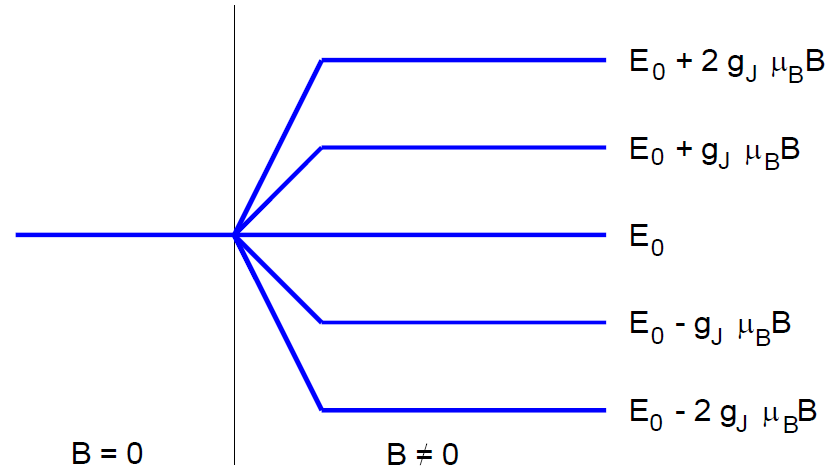
\includegraphics[width=10cm]{images/aufspaltungj2.png}
	\captionof{figure}{Aufspaltung eines Energieniveaus eines Atoms mit der Gesamtdrehimpulsquantenzahl $J=2$. \ref{q:anleitung}}
	\label{fig:aufspaltungj2}
\end{center}

Bei angeregten Atomen können Übergänge zwischen diesen zusätzlichen Energieniveaus angeregt werden, sodass eine einzelne Spektrallinie in mehrere Spektrallinien aufspaltet.
\subsection{Auswahlregeln für Übergänge zwischen zeemanaufgespaltenen Niveaus}
Aus der zeitabhängigen Schrödinger-Gleichung lässt sich eine zeitabhängige Dichteverteilung herleiten, die Schwingung der Elektronen mit der Frequenz
\begin{align}
\nu_{\alpha\beta}=\frac{E_\alpha-E_\beta}{h}
\end{align}
beschreibt.

Außerdem können nur Übergänge mit 
\begin{align}
\Delta m = m_\alpha - m_\beta = -1,\ 0 \text{ oder } 1
\end{align}
angeregt werden.
Dabei sind die bei $\Delta m=0$ emittierten Strahlen linear-polarisiert und parallel zu $\vec{B}$ und die bei $\left|\Delta m \right|=1$ zirkular-polarisiert um die z-Achse.
\subsection{Normale Zeeman-Effekt}
Der Normale Zeeman-Effekt betrachtet den Fall $S=0$. 
Es ergeben sich somit die Energieunterschiede
\begin{align}
\Delta E=m\mu_\indx{B}\hspace{0.2cm}\text{mit }-J\le m \le J \text{.}
\end{align}
Die möglichen Übergänge zwischen $J=2$ und $J=1$ sind in Abbildung \ref{fig:aufspaltungnormal} dargestellt.
\begin{center}
	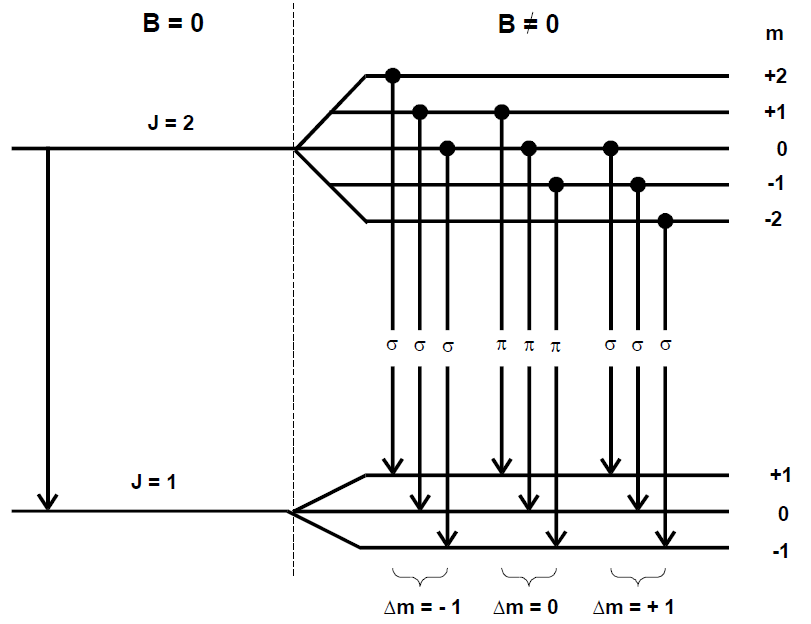
\includegraphics[width=10cm]{images/aufspaltungnormal.png}
	\captionof{figure}{Aufspaltung und Polarisation der Spektrallinien beim normalen Zeeman-Effekt zwischen $J=2$ und $J=1$. \ref{q:anleitung}}
	\label{fig:aufspaltungnormal}
\end{center}
Dabei ist $\Delta m=0$ die $\pi$-Komponente, welche nur bei senkrechter, transversalen Beobachtung zur Feldrichtung mit voller Intensität beobachtbar ist. 
Der Übergang mit $\Delta m=\pm 1$ wird als $\sigma$-Komponente bezeichnet und ist bei jeder Beobachtungsart zu sehen. 
In Abbildung \ref{fig:aufspaltungsbild} ist dieses Aufspaltungsbild visualisiert.
\begin{center}
	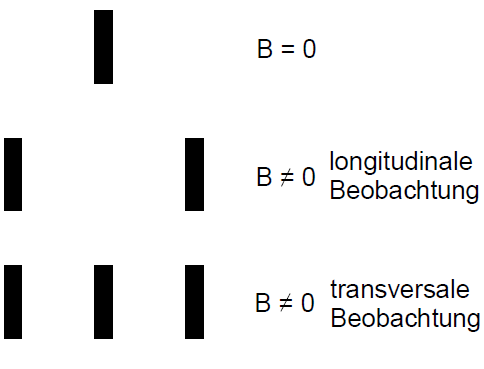
\includegraphics[width=7cm]{images/aufspaltungsbild.png}
	\captionof{figure}{Aufspaltungsbild einer Spektrallinie beim normalen Zeeman-Effekt. \ref{q:anleitung}}
	\label{fig:aufspaltungsbild}
\end{center}

\subsection{Anormale Zeeman-Effekt}
Beim anormalen Zeeman-Effekt wird $S\neq 0$ betrachtet. 
Die Energie zwischen einem Niveau mit Quantenzahlen $L_1$, $S_1$, $J_1$, $m_1$ und einem Niveau mit $L_2$, $S_2$, $J_2$, $m_2$ ist durch 
\begin{align}
E=\left[ m_1 g\left(L_1,S_1,J_1 \right) - m_2 g\left(L_2,S_2,J_2 \right) \right] \mu_\indx{B}B+E_0
\end{align}
gegeben.
Es ergibt sich somit eine linienreichere Aufspaltung, wie in Abbildung \ref{fig:aufspaltunganormal} dargestellt.
\begin{center}
	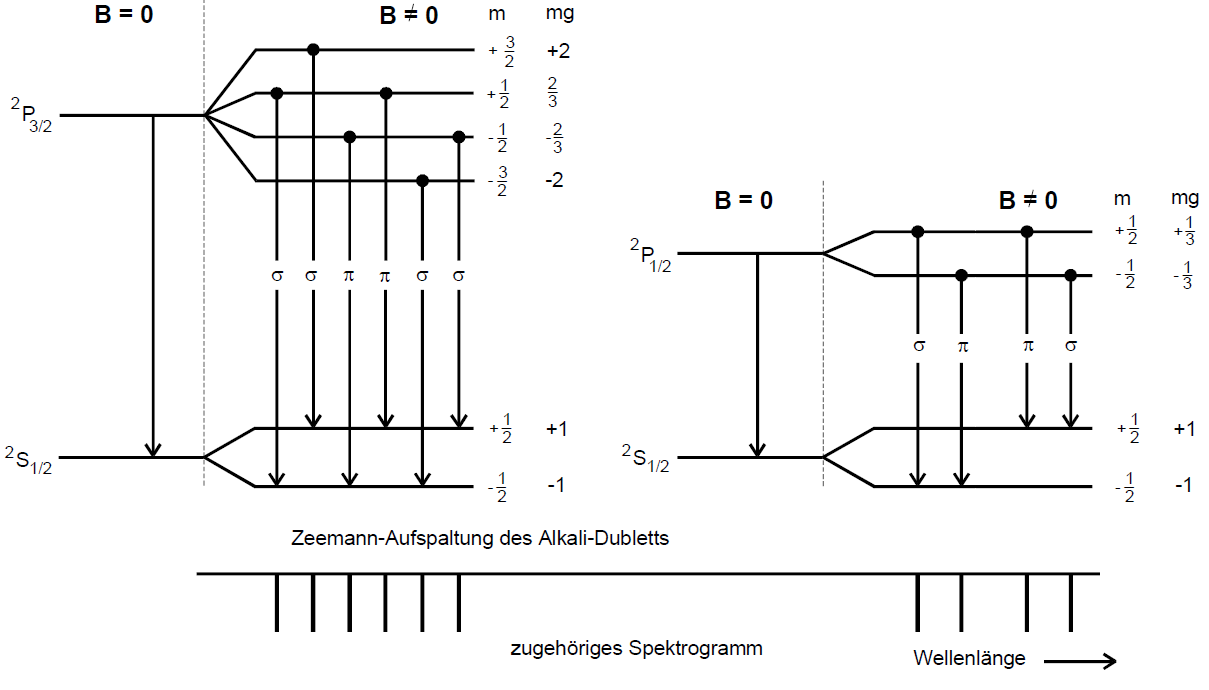
\includegraphics[width=12cm]{images/aufspaltunganormal.png}
	\captionof{figure}{Beispiel einer Linienaufspaltung beim anomalen Zeeman-Effekt. Dargestellt ist die Aufspaltung eines Alkali-Dubletts. \ref{q:anleitung}}
	\label{fig:aufspaltunganormal}
\end{center}
\section{Aufbau}


\section{Durchführung}


\section{Auswertung}


\section{Diskussion}

\section{Quellen}
%\renewcommand{\labelenumi}{\value{enumi}}
\begin{enumerate}[label={[\arabic*]}]
\item \label{q:anleitung} \textbf{Physikalisches Praktikum}, TU Dortmund: \\
\textit{Versuchsanleitung zu Versuch: Röntgenreflektometrie} \\
\url{http://e1.physik.tu-dortmund.de/cms/Medienpool/Downloads/Roentgenreflektometrie_Versuch.pdf} (letzte Version vom 15.02.2017, 12:26)
\end{enumerate}

\end{document}
